
\section{Der Rungesche Approximationssatz}
\label{sec:Runge}

Das große Ziel dieses Kapitels ist der oben genannte
Approximationssatz. Dieser ist eine Verallgemeinerung des Satzes, dass
auf jedem einfach zusammenhängenden Gebiet in $\C$ jede holomorphe
Funktion durch Polynome, also durch ganze Funktionen, approximiert
werden kann.

Auf allgemeinen Riemannschen Flächen muss dazu jedoch "`einfach
zusammenhängende Gebiete"' durch "`Runge-Gebiete"' ersetzt
werden. Später werden wir dieses Resultat verwenden um spezielle
Funktionenfolgen auf Riemannschen Flächen zu konstruieren, die wir
beim Beweis des Riemannschen Abbildungssatzes \ref{thm:rmt} verwenden
werden.

In diesem Kapitel werden direkt die Methoden aus Kapitel
\ref{sec:Weyl} und \ref{sec:frechet} zum Einsatz kommen.

\begin{prop}
  \label{prop:diff-frechet}
  Sei $X$ eine Riemannsche Fläche, $Y \subset X$ offen. 
  Dann besitzen $\diff(Y)$ und $\diff^{0,1}(Y)$ Struktur eines Fr\'echet-Raums.
\end{prop}

\begin{proof}
  Sei für jedes $j \in \N$ die Menge $K_j \subset Y$ kompakt mit $\bigcup_{j \in \N}
  \mathring{K_j} = Y$ und $K_j \subset U_j$, wobei $(U_j, z_j)$ Karten
  sind. Solche $K_j$ können konstruiert werden, da wir im Beweis zu
  Korollar \ref{cor:ausschöpfung-kompakt} eine abzählbare Basis der
  Topologie mit relativ kompakten Teilmengen gefunden haben.
  Für jedes $\nu = (\nu_1, \nu_2)^T \in \N^2$ existiert eine Halbnorm
  \[
  p_{j\nu}: \diff(Y) \ra \R, \quad p_{j\nu}(f) := \|D_j^\nu f\|_{K_j},
  \]
  wobei $D^\nu_j := \left ( \frac{\partial}{\partial x_j} \right
  )^{\nu_1} \left ( \frac{\partial}{\partial y_j} \right )^{\nu_2}$
  mit $z_j = x_j + iy_j$. Dies ist eine abzählbare Familie von
  Halbnormen. Diese können wir verwenden, um eine Topologie auf
  $\diff(Y)$ zu definieren, in dem wir als Basis der Topologie
  endliche Schnitte der Mengen $U(p_{j\nu}, \epsilon, y)$ für
  beliebige $\epsilon > 0$ und $y \in Y$ verwenden (vgl. Definition
  \ref{def:frechet} und Bemerkung \ref{rem:frechet}). Diese Topologie
  ist hausdorffsch, denn falls $0 \neq f \in \diff(Y)$, finden wir
  eine Halbnorm, so dass $\epsilon := p_{j\nu}(f) > 0$. Dann können wir $f$ und 0
  durch die beiden offenen Mengen $U(p_{j\nu}, \frac{\epsilon}{3}, 0)$
  und $U(p_{j\nu}, \frac{\epsilon}{3}, f)$ trennen. Weiterhin ist
  $\diff(Y)$ vollständig bezüglich Konvergenz in allen Halbnormen, da
  alle Ableitung lokal gleichmäßig konvergieren. Damit erfüllt
  $\diff(Y)$ alle Voraussetzungen von Definition \ref{def:frechet}.
  
  Zu guter Letzt behaupten wir nun noch, dass die oben gewählte
  Topologie unabhängig von der gewählten Überdeckung ist. Seien dazu
  $(K_j)$ und $(\tilde K_m)$ zwei Überdeckungen, die den obigen
  Voraussetzungen genügen. Wir bezeichnen mit $(p_{j\nu})$
  bzw. $(\tilde p_{m\nu})$ die zugehörigen Halbnormen. Wir zeigen nun,
  dass $U(p_{j\nu}, \epsilon, f)$ für beliebige $j, \nu \in\N,\
  \epsilon > 0$ und $f \in \diff(Y)$ offen bzgl. der Topologie von
  $(\tilde p_{m\nu})$ ist. Dies genügt bereits, da die Basis der
  Topologie von $(p_{j\nu})$ aus endlichen Schnitten dieser Mengen
  besteht. Wir wissen nun, dass
  \[
  K_j \subset \bigcup_{m=1}^M \mathring{\tilde K}_m \subset \bigcup_{m=1}^M \tilde K_m
  \]
  gilt, da
  $K_j$ kompakt ist. Wir behaupten nun, dass
  \[
  \tilde U := \bigcap_{m=1}^M U(\tilde p_{m\nu}, \epsilon, f) \subset
  U(p_{j\nu}, \epsilon, f)
  \]
  gilt. Sei dazu $g \in \tilde U$. Dann erhalten wir
  \[
  \|D^\nu(g-f)\|_{K_j} \leq \max_{m=1, \dots, M} \|D^\nu(g-f)\|_{\tilde
    K_m} < \epsilon,
  \]
  was die Behauptung zeigt. Für die Rückrichtung vertauschen wir in
  der Argumentation einfach $K_j$ und $\tilde K_j$ und erhalten, dass
  die Topologie unabhängig, von der gewählten Überdeckung ist.
  
  Völlig analog kann die obige Konstruktion auch für $\diff^{0,1}(Y)$
  durchgeführt werden.
\end{proof}

\begin{cor}
  Mit der obigen Topologie ist $\hol(Y) \subset \diff(Y)$ ein
  abgeschlossener Teilraum und die Konvergenz bzgl. dieser Topologie
  stimmt mit der kompakten Konvergenz überein.
\end{cor}

\begin{lemma}
  \label{lemma:kompakter-träger-funktional}
  Sei $Y \subset X$ offen, $X$ eine Riemannsche Fläche. Sei $T \in
  \diff(Y)'$. 
  Dann hat $T$ kompakten Träger, d.h. es existiert ein $K \subset Y$
  kompakt, so dass
  \[
  T[f] = 0 \qquad \forall f \in \diff(Y) \text{ mit } \Supp(f) \subset
  Y \setminus K
  \]
  Das gleiche Resultat gilt für $\diff^{0,1}(Y)$.
\end{lemma}

\begin{proof}
  Aus der Stetigkeit von $T$ folgt die Existenz einer offenen
  Nullumgebung $U \subset \diff(Y)$, so dass
  \[
  |T[f]| < 1 \qquad \forall f \in U
  \]
  Nach Konstruktion der obigen Topologie finden wir ein $\epsilon > 0$
  und endlich viele $j_1, \dots, j_n \in \N$ und $\nu_1, \dots \nu_n
  \in \N^2$, so dass $U(p_{j_1\nu_1}, \epsilon, 0) \cap \dots \cap
  U(p_{j_n\nu_n}, \epsilon, 0) \subset U$. 
  Sei nun  $K := K_{j_1} \cup \dots \cup K_{j_n}$. Wir behaupten, dass
  dies das gesuchte $K$ ist. 
  Dazu wählen wir $f \in \diff(Y)$ mit $\Supp(f) \subset Y \setminus
  K$. Dann gilt für beliebige
  $\lambda > 0$:
  \[
  p_{j_1\nu_1}(\lambda f) = \dots = p_{j_n\nu_n}(\lambda f) = 0
  \]
  Damit liegt $\lambda f \in U$ und es folgt:
  \[
  |T[f]| < \frac1\lambda \qquad \forall \lambda >0
  \]
  und damit $T[f] = 0$.
\end{proof}

\begin{lemma}
  \label{lemma:funktional-explizit}
  Sei $Z \subset X$ offen und $X$ eine Riemannsche Fläche. Sei $S \in
  \diff^{0,1}(X)'$ mit $S[\d[''g]] = 0$ für beliebige $g \in \diff(X)$
  mit $\Supp(g) \Subset Z$. 
  Dann existiert ein $\sigma \in \Omega(X)$ mit $S[\omega] = \iint_Z
  \sigma \wedge \omega$ für jedes $\omega \in \diff^{0,1}(X)$ mit
  $\Supp(\omega) \Subset Z$.
\end{lemma}

\begin{proof}
  Sei $z: U \ra V \subset \C$ eine Karte von $X$ mit $U \subset
  Z$. Wir identifizieren $U$ mit $V$ und können deshalb vom Raum der
  Testfunktionen $\dist(U)$ auf $U$ sprechen. Sei also $\phi \in
  \dist(U)$. Wir bezeichnen mit $\tilde \phi$ jede 1-Form in
  $\dist^{0,1}(X)$, für die $\tilde \phi|_U \equiv \phi \d[\bar z]$ und
  $\tilde \phi |_{X \setminus U} \equiv 0$ gilt. 
  Damit können wir ein $S_U \in \dist(U)'$ definieren:
  \[
  S_U: \dist(U) \ra \C, \phi \mapsto S[\tilde \phi]
  \]
  Diese verschwindet auf allen Funktionen $\phi = \frac{\partial
    g}{\partial \bar z}$, $g \in \dist(U)$, denn $S_U[\phi] = S[\tilde
  \phi] = S[ \frac{\partial g}{\partial \bar z} \d[\bar z]] =
  S[\d[''g]] = 0$ nach Voraussetzung. Das bedeutet aber, dass
  $\frac{\partial S_U}{\partial \bar z} = 0$ gilt und aus Korollar
  \ref{cor:hol-dist} erhalten wir ein $h \in \hol(U)$:
  \[
  S[\tilde \phi] = \iint_U h(z) \phi(z) \d[z] \wedge \d[\bar z] \qquad
  \forall \phi \in \dist(U)
  \]
  Setzen wir nun $\sigma_U := h \d[z]$, so folgt
  \[
  S[\omega] = \iint_U \sigma_u \wedge \omega \qquad \omega \in
  \dist^{0,1}(U) \text{ und } \Supp(\omega) \Subset U
  \]
  Führen wir die gleiche Konstruktion auf einer zweiten Karte (z', U')
  durch und gilt außerdem noch, dass $\Supp(\omega) \Subset U'$, so
  erhalten wir
  \[
  \iint_U \sigma_U \wedge \omega = S[\omega] = \iint_{U'} \sigma_{U'}
  \wedge \omega \qquad \forall \omega \in \diff^{0,1}(X) \text{ und }
  \Supp(\omega) \Subset U \cap U'
  \]
  und damit $\sigma_U|_{U \cap U'} \equiv \sigma_{U'}|_{U \cap
    U'}$. Also können wir alle $\sigma_U$ zu einer globalen 1-Form
  $\sigma \in \Omega(Z)$ verkleben und es folgt
  \[
  S[\omega] = \iint_Z \sigma \wedge \omega \qquad \forall \omega \in
  \diff^{0,1}(X) \text{ mit } \Supp(\omega) \Subset U,
  \]
  wobei $U$ eine Koordinatenumgebung darstellt. 
  Wählen wir nun ein beliebiges $\omega \in \diff^{0,1}(X)$ mit
  $\Supp(\omega) \Subset Z$, so können wir eine Partition der 1
  wählen, so dass $\omega = \sum_{j=1}^n \omega_J$ mit
  $\Supp(\omega_j) \Subset U_j$. Dabei sind die $U_j$
  Koordinatenumgebungen. 
  Zu guter Letzt erhalten wir damit
  \[
  S[\omega] = \sum_{j=1}^n S[\omega_j] = \sum_{j=1}^n \iint_Z \sigma
  \wedge \omega_j = \iint_Z \sigma \wedge \omega.
  \]
\end{proof}

\begin{thm}
  \label{thm:runge-dicht}
  Sei $Y \Subset X$ eine offene Runge-Teilmenge und $X$ eine nicht
  kompakte Riemannsche Fläche. 
  Dann liegt $\im( \hol(Y') \ra \hol(Y))$ für beliebige $Y' \Subset X$
  offen und $Y \subset Y'$ bzgl. kompakter Konvergenz dicht in $\hol(Y)$.
\end{thm}

\begin{proof}
  Sei $\beta: \diff(Y') \ra \diff(Y)$ die Einschränkungsabbildung. Wir
  verwenden Korollar \ref{cor:frechet-dicht}. Dazu müssen wir zeigen, dass für $T \in
  \diff(Y)'$ mit $T_{\beta(\hol(Y'))} \equiv 0$ auch $T|_{\hol(Y)}
  \equiv 0$ gilt. 
  Nach \cite[Kor. 14.16]{For} existiert zu jedem $\omega \in \diff^{0,1}(X)$ ein $f \in
  \diff(Y')$ mit $\d[''f] = \omega|_{Y'}$. 
  Dies erlaubt uns die Definition von $S: \diff^{0,1}(X) \ra \C, \quad
  S[w] := T[f|_Y]$. Diese Definition ist unabhängig von $f$, denn für
  ein $g \in \diff(Y')$ mit $\d[''g] = \omega|_{Y'}$, dann ist $f-g
  \in \hol(Y')$ und deshalb $T[(f-g)|_Y] = 0$ nach der Voraussetzung,
  dass $T|_{\beta(\hol(Y'))} \equiv 0$. 
  Als nächstes wollen wir zeigen, dass $S$ stetig ist. 
  Dazu betrachten wir zunächst
  \[
  V := \{ (\omega, f) \in \diff^{0,1}(X) \times \diff(Y') \mid \d[''f] = \omega|_{Y'} \}.
  \]
  Nun haben wir
  sowohl $\diff(Y')$, als auch $\diff^{0,1}(Y')$ mit der Topologie
  eines Fr\'echet-Raums ausgestattet. Wählen wir eine Überdeckung von
  $Y'$ durch Kompakta wie im Beweis von Proposition
  \ref{prop:diff-frechet} und eine Folge $(f_n)_{n\in \N} \subset
  \diff(Y')$, die bzgl. der Fr\'echet-Topologie gegen $f \in \diff(Y')$
  konvergiert, so gilt auf den Kompakta, dass $(f_n)_{n\in \N}$ glatt
  gegen $f$ konvergiert, d.h. heißt aber, dass bezüglich den Karten
  auch die Folge $\left(\frac{\partial f_n}{\partial \bar z} \right
  )_{n \in\N}$ glatt gegen $\frac{\partial f}{\partial \bar
      z}$ konvergiert. Mit anderen Worten konvergiert
    $(\d[''f_n])_{n\in \N}$ gegen $\d[''f]$. Also ist 
  $\d['']: \diff(Y') \ra \diff^{0,1}(Y')$ stetig und es folgt, dass $V
  \subset \diff^{0,1}(X) \times \diff(Y')$ abgeschlossen und somit
  nach den Sätzen \ref{thm:frechet-abgeschlossen} unf \ref{thm:frechet-summe} ein
  Fr\'echet-Raum ist.
  
  Nach \cite[Kor. 14.16]{For} ist $\pi_1: V \ra \diff^{0,1}(X)$
  surjektiv und stetig. Es folgt aus dem Satz über die offene
  Abbildung, dass $\pi_1$ offen ist.
  Weiterhin ist $\beta \circ \pi_2 : V \ra \diff(Y)$ stetig. Da nun
  auch noch das folgende Diagramm kommutiert,
  \begin{center}
    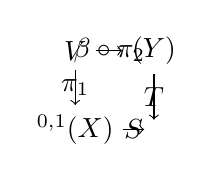
\begin{tikzpicture}
      \node (V) {$V$};
      \node (ey) [right of=V] {$\diff(Y)$};
      \node (ex) [below of=V] {$\diff^{0,1}(X)$};
      \node (C) [right of =ex] {$\C$};
      \draw[->] (V) to node{$\beta \circ \pi_2$} (ey);
      \draw[->] (V) to node{$\pi_1$} (ex);
      \draw[->] (ey) to node{$T$} (C);
      \draw[->] (ex) to node{$S$} (C);
    \end{tikzpicture}
  \end{center}
  folgt die Stetigkeit von $S$.

  Das Lemma \ref{lemma:kompakter-träger-funktional} liefert
  \begin{itemize}
  \item ein kompaktes $K \subset Y$ mit $T[f] = 0$ für jedes $f \in
    \diff(Y)$ mit $\Supp(f) \subset Y \setminus K$ und
  \item ein kompaktes $L \subset X$ mit $S[\omega] = 0$ für jedes
    $\omega \in \diff^{0,1}(X)$ mit $\Supp(\omega) \subset X\setminus L$
  \end{itemize}
   Sei $g \in \diff(X)$ mit $\Supp(g) \Subset X \setminus K$. Dann ist
   $S[\d[''g]] = T[g|_Y]  = 0$. Lemma \ref{lemma:funktional-explizit}
   gibt uns dann ein $\sigma \in \Omega(X\setminus K)$ mit
   \[
   S[\omega] = \iint_{X \setminus K}\sigma \wedge \omega \qquad
   \forall \omega \in \diff^{0,1}(X) \text{ mit } \Supp(\omega)
   \Subset X\setminus K
   \]
   Aufgrund des kompakten Trägers von $S$ muss $\sigma|_{X \setminus
     (K \cup L)} \equiv 0$ gelten. 
   Nun ist jede Zusammenhangskomponente von $X \setminus \runge(K)$
   nicht relativ kompakt. 
   Wir behaupten, dass jede Zusammenhangskomponente von $X \setminus
   \runge(K)$ die Menge $X \setminus (K \cup L)$ schneidet.
   Angenommen es gäbe eine Zusammenhangskomponente $U \subset X
   \setminus \runge(K)$ mit $U \cap X \setminus ( K \cup L) =
   \varnothing$. Dann gälte $U \subset K \cup L$, also wäre $U$ relativ
   kompakt. Ein Widerspruch. Also schneiden alle
   Zusammenhangskomponenten $X \setminus (K \cup L)$ und aus dem
   Identitätssatz folgt:
   \begin{align}
   \sigma|_{X \setminus \runge(K)} \equiv 0 \label{eq:runge}
   \end{align}
   Das bedeutet, dass $S[\omega] = 0$ für jedes $\omega \in
   \diff^{0,1}(X)$ mit $\Supp(\omega) \Subset X \setminus
   \runge(K)$.

   Sei nun $f \in \hol(Y)$. Wir wollen zeigen, dass $T[f] = 0$. \\
   Zunächst gilt $\runge(K) \subset \runge(Y) = Y$. Nun können wir
   eine offene Mengen $U, V$ finden, die $ \runge(K) \subset U
   \subsetneq V \subset Y$ erfüllen. Nach dem Lemma von Urysohn
   (vgl. \cite[Satz 12.2]{Jam}) finden
   wir eine stetige Funktion $\phi: X \ra \R$, die $\phi|_U \equiv 1$
   und $\phi|_{X \setminus \bar V} \equiv 0$ erfüllt. Durch eine geeignete Glättung
   dieser Funktion $\phi$ erhalten wir ein glattes $\tilde \phi \in
   \diff(X)$ und offene Mengen $\runge(K) \subset \tilde U \subset U$
   und $U \subset \tilde V \subset V$, so dass $\tilde \phi|_{\tilde
     U} \cong 1$ und $\tilde \phi|_{X \setminus \tilde {\bar V}} \cong
   0$ gilt. Setzen wir $ g := f \cdot \tilde \phi$, so gilt
   $f \equiv g$ in einer Umgebung von $\runge(K)$ und $\Supp(g) \Subset Y$.
   Also liegt $\Supp(f - g|_Y) \subset Y \setminus K$, somit gilt $T[f- g|_Y] = 0$
   und schlußendlich $T[f] = T[g|_Y] = S[\d[''g]]$. 
   Nun ist aber $g$ in einer Umgebung von $\runge(K)$ holomorph, was
   nichts anderes bedeutet als, dass $\Supp(\d[''g]) \Subset X \setminus
   \runge(K)$ gilt.
   Mit \eqref{eq:runge} folgt
   \[
   T[f] = T[g|_f] = S[\d[''g]] = 0
   \]
\end{proof}

\begin{thm}[Rungescher Approximationssatz]
  \label{thm:runge}
  Sei $X$ eine nicht kompakte Riemannsche Fläche, $Y \subset X$ eine
  offene Runge-Teilmenge.
  Dann kann jede holomorphe Funktion auf $Y$ auf beliebigen Kompakta
  gleichmäßig durch holomorphe Funktionen auf ganz $X$ approximiert werden.
\end{thm}

\begin{proof}
  \begin{description}
  \item[Fall $Y \Subset X$:] Seien $f \in \hol(Y)$, $K \subset Y$
    kompakt und $\epsilon > 0$ gegeben. 
    Aus dem Beweis von Satz \ref{thm:Ausschöpfung-Runge} erhalten wir
    eine Ausschöpfung$Y_1
    \Subset Y_2 \Subset \dots$ von $X$ mit $Y_0 := Y \Subset Y_1$. 
    Nach Satz \ref{thm:runge-dicht} existiert ein $f \in \hol(Y_1)$
    mit
    \[
    \|f_1 - f\|_K < 2^{-1} \epsilon
    \]
    Induktiv erhalten wir aus Satz \ref{thm:runge-dicht} eine Folge
    von Funktionen $f_n \in \hol(Y_n)$ mit
    \[
    \|f_n - f_{n-1}\|_{\bar Y_{n-2}} < 2^{-n} \epsilon \qquad \forall
    n \geq 2
    \]
    Nun gilt für beliebige $n \in \N$:
    \[
    \|f_{\nu + k} - f_{\nu} \|_{Y_n} \leq \epsilon 2^{-\nu} \sum_{\mu
      = 0}^k 2^{-\mu} \leq  \epsilon 2^{-(\nu+1)} \xrightarrow{\nu \ra
      \infty} 0 \qquad \forall \nu > n
    \]
    Also konvergiert $(f_\nu)_{\nu > n}$ gleichmäßig auf $Y_n$ für
    jedes $n \in \N$ und damit existiert ein $F \in \hol(X)$, so dass
    $f_\nu \rightrightarrows F$ auf jedem $Y_n$. Eingesetzt folgt
    \begin{align*}
      \|F - f\|_K & \leq \|F - f_n\|_{Y_n} + \sum_{k=1}^n \|f_k -
      f_{k-1}\|_{\bar Y_{k-2}} \\
      & < \|F - f_n \|_{Y_n} + \epsilon \sum_{k=1}^n 2^{-k} \\
      & \xrightarrow{n \ra \infty} \epsilon.
    \end{align*}
  \item[Fall $Y \subset X$ nicht relativ kompakt:] Auch hier wählen
    wir $f \in \hol(Y)$, $K \subset Y$ kompakt und $\epsilon > 0$. \\
    In diesem Fall können wir nach Lemma \ref{lemma:komp-enthalten}  $L \subset Y$ kompakt finden mit $K \subset
    \mathring L$. Dann folgt aus Lemma \ref{lemma:zwischen-runge} die Existenz einer
    offenen Runge-Teilmenge
    $\tilde Y \subset X$ mit $K \subset \tilde Y \subset L$. 
    Damit ist $\tilde Y \Subset X$ und $f$ kann als Funktion von
    $\hol(\tilde Y)$ aufgefasst werden und schlussendlich können wir
    den obigen Fall anwenden und erhalten ein $F \in \hol(X)$ mit
    $\|f|_{\tilde Y} - F\|_K = \|f - F\|_K < \epsilon$.
  \end{description}
\end{proof}

\begin{thm}
  \label{thm:h-hol}
  Sei $X$ eine nicht kompakte Riemannsche Fläche und $\omega \in
  \diff^{0,1}(X)$. Dann existiert ein $f \in \diff(X)$, so dass
  \[
  \d[''f] = \omega
  \]
  gilt.
\end{thm}

\begin{proof}
  Sei
  \[
  Y_0 \subseteq Y_1 \subseteq \dots
  \]
  eine Ausschöpfung von $X$ durch Runge-Gebiete. Wir wollen nun eine
  Folge von $f_n \in \diff(Y_n)$, so dass die Bedingungen
  \begin{enumerate}
  \item $\d[''f_n] = \omega|_{Y_n}$ und
  \item $\|f_{n+1} - f_n \|_{Y_{n-1}} \leq 2^{-n}$
  \end{enumerate}
  erfüllt sind. Wir gehen dazu induktiv vor. Zunächst existiert nach
  \cite[Kor. 14.16]{For} ein $f_0 \in \diff(Y_0)$, so dass $\d[''f_0]
  = \omega|_{Y_0}$ gilt. Seien nun $f_0, \dots, f_n$ bereits
  konstruiert. Erneut nach \cite[Kor. 14.16]{For} erhalten wir ein
  $g_{n+1} \in \diff(Y_{n+1})$, so dass $\d[''g_{n+1}] =
  \omega|_{Y_{n+1}}$ erfüllt. Dann gilt aber auf $Y_n$ die Gleichung
  \[
  \d['' g_{n+1}] = \d['' f_n],
  \]
  was nichts anderes bedeutet, als dass $g_{n+1} - f_n$ holomorph auf
  $Y_n$ ist. Nach dem Rungeschen Approximationssatz \ref{thm:runge}
  existiert ein $h \in \hol(Y_{n+1})$, so dass
  \begin{align}
  \|(g_{n+1} - f_n) - h\|_{Y_{n-1}} \leq 2^{-n} \label{eq:app}
  \end{align}
  gilt. Definieren wir $f_{n+1} := g_{n+1} - h$, so erfüllt $f_{n+1}$
  immer noch die erste und dank \eqref{eq:app} auch die zweite
  Bedingung.

  Nun definieren wir
  \[
  f(z) := \lim_{n \ra \infty} f_n(z).
  \]
  Die Funktion $f$ ist wohldefiniert, da jedes $z \in X$ in fast allen
  $Y_n$ enthalten ist. Weiterhin können wir auf $Y_{n-1}$ die Darstellung
  \[
  f = f_n + \sum_{k=n}^\infty (f_{k+1} - f_k) =: f_n + F_n
  \]
  wählen. Nun konvergiert $F_n$ gleichmäßig auf $Y_{n-1}$ und ist deshalb
  dort holomorph. Also ist $f$ glatt auf $Y_n$ für beliebige $n \in
  \N$, in anderen Worten ist $f \in \diff(X)$. Weiterhin gilt
  \[
  \d[''f] = \d['' f_n] = g
  \]
  auf $Y_{n-1}$ für beliebige $n \in \N$ und damit $\d[''f] = g$ auf $X$.
\end{proof}

\begin{cor}
  \label{cor:h-hol}
  Sei $X$ eine nicht kompakte Riemannsche Fläche. Dann ist $H^1(X,
  \hol) = 0$.
\end{cor}

\begin{proof}
  Aus dem Satz von Dolbeault (vgl. \cite[Satz 15.14]{For}) folgt die
  Gleichung
  \[
  H^1(X, \hol) \cong \quot{\diff^{0,1}(X)}{\d['' \diff(X)]}.
  \]
  Satz \ref{thm:h-hol} besagt nun aber $\diff^{0,1}(X) =
  \d[''\diff(X)]$, was die Behauptung zeigt.
\end{proof}

%%% Local Variables: 
%%% mode: latex
%%% TeX-master: "../Bachelor"
%%% End: 
